\section{Inhomogeneous Erd\"os-R\'enyi Random Networks}
\label{sec:ch5:ier}


Now that you've learned about the $ER_n(p)$, $SBM_n(\vec z, B)$, and $RDPG_n(X)$ random networks, it's time to figure out why we keep using coin flips! To this end, we will learn about the most general model for an independent edge random network, the Inhomogeneous Erdos Renyi (IER) Random Network.

\subsection{The Inhomogeneous Erdos-Renyi (IER) Random Network Model is parametrized by a matrix of independent-edge probabilities}

The IER random network is the most general random network model for a binary graph. The way you can think of the IER random network is that a probability matrix $P$ with $n$ rows and $n$ columns defines each of the edge-existence probabilities for pairs of nodes in the network. This is called the \textit{probability matrix} for the independent-edge random network model. For each pair of nodes $i$ and $j$, you have a unique coin which has a $p_{ij}$ chance of landing on heads, and a $1 - p_{ij}$ chance of landing on tails. If the coin lands on heads, the edge between nodes $i$ and $j$ exists, and if the coin lands on tails, the edge between nodes $i$ and $j$ does not exist. This coin flip is performed independently of the coin flips for all of the other edges. If $\mathbf A$ is a random network which is $IER$ with a probability matrix $P$, we say that $\mathbf A$ is an $IER_n(P)$ random network.

\subsubsection{Generating a sample from an $IER_n(P)$ random network}

As before, we develop a procedure in Algorithm \ref{alg:ch5:ier} to produce for you a network $A$, which has nodes and edges, where the underlying random network $\mathbf A$ is an $IER_n(P)$ random network.

\begin{algorithm}[h]\caption{Simulating a sample from an $IER_n(P)$ random network}
\label{alg:ch5:ier}
\SetAlgoLined
\KwData{$n$ a number of nodes \newline$P$ a probability matrix with $n$ rows and $n$ columns}
\KwResult{The adjacency matrix of a sample from the random network.}

\For{$i$ in $1$:$n$} {
    \For{$j > i$} {
        Obtain a weighted coin $(i,j)$ which has a probability $p_{ij}$ of landing on heads, and a $1 - p_{ij}$ probability of landing on tails.

        Flip the $(i,j)$ coin, and if it lands on heads, the corresponding entry $a_{ij}$ in the adjacency matrix is $1$. If the coin lands on tails, the corresponding entry $a_{ij}$ is $0$. 

        Set $a_{ji} = a_{ij}$.
    }
}
\Return{$A$}
\end{algorithm}

\begin{floatingbox}[h]\caption{$IER_n(P)$ and $SBM_n(\vec z, B)$ equivalence}
Notice that the model that we described for an $IER_n(P)$ random network is, in fact, equal to a very uninformative $SBM_n(\vec z, B)$ random network. If the network is simple, we could simply assign each node to its own community; e.g., the number of communities is $n$. Then, we can just let the block matrix $B$ be equal to the probability matrix $P$. However, if the number of communities is not equal to the number of nodes, this is not generally the case.
\end{floatingbox}

Let's put this in practice. Let's first generate a probability matrix that is sufficiently unnecessarily complicated that we couldn't capture it with the any Erd\"os R\'enyi, Stochastic Block Model with the fewer communities than nodes, nor an RDPG:

\begin{lstlisting}[style=python]
import numpy as np
from graphbook_code import heatmap

def my_unit_circle(r):
   d = 2*r + 1
   rx, ry = d/2, d/2
   x, y = np.indices((d, d))
   return (np.abs(np.hypot(rx - x, ry - y)-r) < 0.5).astype(int)

def add_smile():
    Ptmp = np.zeros((51, 51))
    Ptmp[2:45, 2:45] = my_unit_circle(21)
    mask = np.zeros((51, 51), dtype=bool)
    mask[np.triu_indices_from(mask)] = True
    upper_left = np.rot90(mask)
    Ptmp[upper_left] = 0
    return Ptmp
    
def smiley_prob(upper_p, lower_p):
    smiley = add_smile()
    P = my_unit_circle(25)
    P[5:16, 25:36] = my_unit_circle(5)
    P[smiley != 0] = smiley[smiley != 0]
    
    mask = np.zeros((51, 51), dtype=bool)
    mask[np.triu_indices_from(mask)] = True
    P[~mask] = 0
    P = (P + P.T - np.diag(np.diag(P))).astype(float)
    P[P == 1] = lower_p
    P[P == 0] = upper_p
    return P

P = smiley_prob(.95, 0.05)
heatmap(P, vmin=0, vmax=1, title="Probability matrix $P$")
\end{lstlisting}

The probability matrix is plotted in Figure \ref{fig:ch5:ier}(A). Next, we can generate a random sample of the $IER_n(P)$ random network:

\begin{lstlisting}[style=python]
from graspologic.simulations import sample_edges

A = sample_edges(P, directed=False, loops=False)
heatmap(A.astype(int), title="$IER_n(P)$ sample")
\end{lstlisting}

The heatmap is shown in Figure \ref{fig:ch5:ier}(B). We used this example to show you the key idea behind the IER Network's probability matrix is simple: the entries can really be anything as long as they are probabilities (between $0$ and $1$), and the resulting matrix is symmetric (in the case of undirected networks). There are no additional requirements nor parameters to add structure to the network.

\begin{figure}
    \centering
    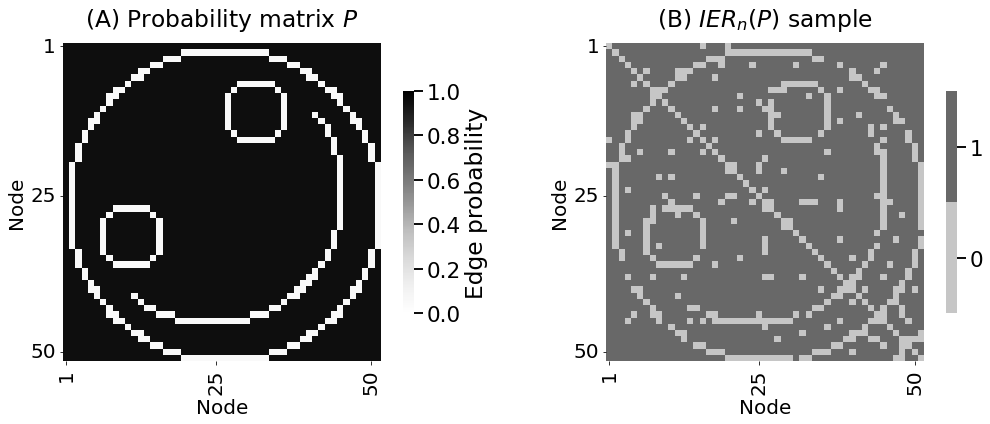
\includegraphics[width=\linewidth]{representations/ch5/Images/ier.png}
    \caption[$IER_n(P)$ parameters]{\textbf{(A)} the probability matrix for the $IER_n(P)$ random network. \textbf{(B)} an adjacency matrix sampled from the $IER_n(P)$ random network.}
    \label{fig:ch5:ier}
\end{figure}

\subsection{Unifying Independent-Edge Random Network Models}

The class of models that we have learned about so far are more generally known as independent-edge random networks \cite{Athreya2017Jan}. As it turns out, just like the $ER_n(p)$ random network was a special case of the $SBM_n(\vec z, B)$ random network, there are many other relationships that we can study as well. In this sense, we will study the ``hierarchy of network models''. A model is said to be more complex than a second model if we can generate the parameters of the first model using the parameters of the second model, but we cannot necessarily do the reverse.

\subsubsection{All independent-edge random networks are IER networks}
\label{sec:ch5:ier:ier_generalises}
The $IER_n(P)$ random network is more complex than every model that we have learned to date.
\begin{enumerate}
    \item Erd\"os R\'enyi with probability $p$: all entries $p_{ij}$ of $P$ can just be set equal to $p$,
    \item Stochastic block model with community assignment vector $\vec z$ and block matrix $B$: construct the probability matrix $P$ such that $p_{ij} = b_{z_iz_j}$ of the block matrix $B$ where the communities of nodes $i$ and $j$ are $z_i$ and $z_j$, respectively.
    \item Random Dot Product Graph with latent position matrix $X$: Let $P$ such that $P = XX^\top$. Note that the entries of $P$ by definition of matrix multiplication will be $p_{ij} = \vec x_i^\top \vec x_j$, which was exactly the relationship that we established in Section \ref{sec:ch5:rdpg}.
\end{enumerate}

\paragraph{How do we generate a probability matrix from a $SBM_n(\vec z, B)$?}
\label{sec:ch5:ier:sbm_pmtx}
One thing that will come up frequently over the course of this book is that we will need to sometimes programmatically generate the probability matrix directly (rather than just using the community assignment vector $\vec z$ and the block probability matrix $B$). This isn't too difficult to do, and some pseudocode is outlined in Algorithm \ref{alg:ch5:sbm_pmtx}.

\begin{algorithm}[h]\caption{Generating a probability matrix for a $SBM_n(\vec z, B)$ random network}
\label{alg:ch5:sbm_pmtx}
\SetAlgoLined
\KwData{$\vec z$ a community assignment vector for each of the $n$ nodes to one of $K$ communities\newline $B$ a block matrix with $K$ rows and $K$ columns}
\KwResult{The probability matrix associated with the $SBM_n(\vec z, B)$.}

Construct a matrix $C$ with $n$ rows and $K$ columns; one row for each node, and one column for each community.

\For{$i$ in $1$:$n$} {
    \For{$k$ in $1$:$K$} {
        If $z_i = k$, let $c_{ik} = 1$. If $z_i \neq k$, let $c_{ik} = 0$.
    }
}

Let $P = CBC^\top$.
\end{algorithm}

Let's break down exactly how this works. The matrix $C$ is better known as a one-hot encoding of the matrix $\vec z$. When we multiply $CB$, the matrix product will be the $n \times k$ matrix:
\begin{align*}
    (CB)_{ik} = \sum_{l = 1}^Kc_{il} b_{lk}.
\end{align*}
However, we know that $c_{il} = 1$ if $z_i = l$, and $0$ otherwise. So for each entry:
\begin{align*}
    (CB)_{ik} = b_{z_i k}
\end{align*}
This matrix is going to end up looking something like this:
\begin{align*}
    CB = \begin{bmatrix}
        b_{z_i1} & \hdots & 
        b_{z_iK} \\
        \vdots & \ddots & \vdots \\
        b_{z_n1} & \hdots & b_{z_n K}
    \end{bmatrix}.
\end{align*}
So each row of $CB$ corresponds to a single node $i$ in the network, identifies the community of that node, and then ``extracts'' from the block matrix all of the other communities that another node $j$ could possibly be in. When we right-multiply by $C^\top$, what we get is:
\begin{align*}
    (CBC^\top)_{ij} = \sum_{l = 1}^Kc_{jl}b_{z_il}.
\end{align*}
As before, $c_{jl} = 1$ if $z_j = l$, and $0$ otherwise. So for each entry:
\begin{align*}
    p_{ij} = (CBC^\top)_{ij} = b_{z_i z_j}. \numberthis \label{eqn:ch5:ier:sbm_p}
\end{align*}
Notice that this aligns exactly with the result that we obtained in Section \ref{sec:ch5:ier:ier_generalises}.

Let's work through this example programmatically, because it comes up a few times over the course of the book. Let's imagine that we have $50$ nodes, of which the first $25$ are in community one and the second $25$ are in community two. The code to do this conversion looks like this:

\begin{lstlisting}[style=python]
def ohe_comm_vec(z):
    """
    A function to generate the one-hot-encoded community
    assignment matrix from a community assignment vector.
    """
    K = len(np.unique(z))
    n = len(z)
    C = np.zeros((n, K))
    for i, zi in enumerate(z):
        C[i, zi - 1] = 1
    return C

def generate_sbm_pmtx(z, B):
    """
    A function to generate the probability matrix for an SBM.
    """
    C = ohe_comm_vec(z)
    # probability matrix
    return C @ B @ C.T

# the community assignment vector
z = [1 for i in range(0, 25)] + [2 for i in range(0, 25)]
# block matrix
B = np.array([[0.6, 0.3], [0.3, 0.6]])
# probability matrix
P = generate_sbm_pmtx(z, B)
\end{lstlisting}

The relationship between the community assignment vector, the community assignment matrix, the block matrix, and the probability matrix is illustrated in Figure \ref{fig:ch5:ier:sbm}.

\begin{figure}
    \centering
    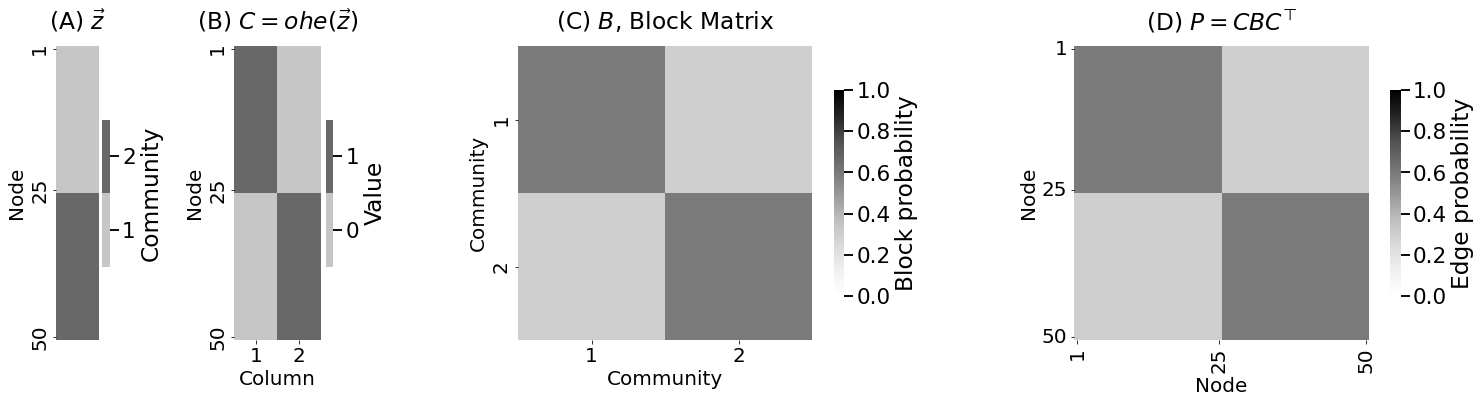
\includegraphics[width=\linewidth]{representations/ch5/Images/sbm_prob.png}
    \caption[Deriving probability matrix for $SBM_n(\vec z, B)$ random network.]{\textbf{(A)} the community assignment vector $\vec z$ and \textbf{(B)} the community assignment matrix $C$. Notice that each node has a value of $1$ in the corresponding column in which the node is a community. The first 25 nodes have a value of $1$ in column $1$, and the second $25$ nodes have a value of $1$ in column $2$. \textbf{(C)} the block matrix. \textbf{(D)} the probability matrix for each node pair.}
    \label{fig:ch5:ier:sbm}
\end{figure}

\subsubsection{What is the difference in complexity between the $SBM_n(\vec z, B)$ and $RDPG_n(X)$?}
\label{sec:ch5:ier:rdpg_sbm}

It is rather trivial to conclude that $RDPG_n(X)$ are more complex than $ER_n(p)$ random networks. Choose $X$ to be a matrix with $n$ rows and $1$ column, where every entry is $\sqrt p$). However, it is not at all obvious the relationship between the $SBM_n(\vec z, B)$ random networks and a $RDPG_n(X)$. 

When the number of communities is less than the number of nodes, the street example that we gave in Section \ref{sec:ch5:rdpg} is sufficient to prove that $RDPG_n(X)$ is not a special case of $SBM_n(\vec z, B)$ with $K < n$; that is, there are $RDPG_n(X)$ random networks that are not $SBM_n(\vec z, B)$ random networks. The street example cannot be captured with an SBM unless we take the number of communities equal to the number of nodes. You will better understand why this is the case in Section \ref{sec:ch5:psd_block:same_lp}.

Notice, on the other hand, that if we are given a probability matrix $P$, that if there exists a matrix $X$ where $P = XX^\top$, that we could build an $RDPG_n(X)$ random network by using the matrix $X$ as the latent position matrix. This condition is equivalent to stating that $P$ must be positive semi-definite \cite{Athreya2017Jan,Rubin2022Sep}.

In the case of an $SBM_n(\vec z, B)$ random network, the probability matrix $P = CBC^\top$ will be positive semi-definite whenever $B$ is positive semi-definite \cite{Chung2021Mar,Athreya2017Jan}. This would mean that $B$ can be written as the product of a matrix $\sqrt B$ and its transpose $\sqrt B^\top$. In this case, if we took the latent position matrix $X$ to be $C\sqrt B$, we would get that:
\begin{align*}
    XX^\top &= C\sqrt B\sqrt B^\top C^\top \numberthis\label{eq:ch5:ier:sbm_rdpg}\\
    &= CBC^\top,
\end{align*}
which is the probability matrix of a $SBM_n(\vec z, B)$ random network. This shows that if every SBM with a block matrix that positive semi-definite can be transformed to an RDPG, so the $RDPG_n(X)$ is more complex than the $SBM_n(\vec z, B)$ with a positive semi-definite block matrix and a number of communities less than the number of nodes. 

Unfortunately, going into too much more mathematical depth about the concept of positive semi-definiteness would get overly mathematical, so we will leave you with some practical guidance on a several types of block matrices that are positive semi-definite in Section \ref{sec:ch5:psd_block}. If you want more technical depth on positive semi-definite matrices, we would recommend a matrix analysis book, like \cite{Horn2012Oct}. To check a given block matrix \texttt{B} for positive semi-definiteness, you can use this utility, which builds upon concepts from \cite{Horn2012Oct}:

\begin{lstlisting}[style=python]
def block_mtx_psd(B):
    """
    A function which indicates whether a block matrix
    B is positive semi-definite.
    """
    return np.all(np.linalg.eigvals(B) >= 0)
block_mtx_psd(B)
# True
\end{lstlisting}

Consequently, this will tell you whether your $SBM_n(\vec z, B)$ random network can be described by an $RDPG_n(X)$ random network.

\paragraph{Is there a more general RDPG where we don't need this ``positive semi-definite'' restriction?}
\label{sec:ch5:ier:grdpg}
The answer to this question is yes, there is a generalization of an RDPG where all stochastic block models can be captured: the aptly-named Generalized Random Dot Product Graph \cite{Rubin2022Sep}, or gRDPG. This generalization allows you to capture block matrices which are not positive semi-definite, also known as indefinite. This model underlies the theoretical motivation for many techniques that we will describe in Chapter \ref{sec:ch6}. The technical and theoretical details of these types of RDPGs are beyond the scope of this book, although some statistical formalization is provided in Appendix \ref{app:ch12:rdpg}.

\subsubsection{The hierarchy of independent-edge random network models}

In general, the ``hierarchy of complexity'' of our network models is shown in Figure \ref{fig:ch5:hierarchy}. The circles indicate the breadth of problems that the particular network model can be used to describe. If one model is entirely contained within another, that every random network described by the contained model can also be described by the subsuming model (where the reverse is not true). If the two models overlap, it means that some random networks described by one of the models can also be described by the other model, but not necessarily always.

To succinctly summarize what we've learned so far:
\begin{enumerate}
    \item $ER_n(p)$ random networks are less complex than $SBM_n(\vec z, B)$ with $K < n$: choose a $1$-community $SBM$ with a block matrix of $B = [p]$.
    \item $ER_n(p)$ random networks are less complex than $RDPG_n(X)$: could choose the latent position matrix to be a $1$-column matrix whose only entry is $\sqrt p$.
    \item $SBM_n(\vec z, B)$ with $K < n$ and positive semi-definite $B$ is less complex than $RDPG_n(X)$: Let $\sqrt B$ be the square-root of the matrix $B$, and $C$ the one-hot encoding of the matrix $\vec z$. Take $X = C\sqrt B$.
    \item $SBM_n(\vec z, B)$ with $K < n$ and indefinite $B$ is not describable with $RDPG_n(X)$: indefinite $B$ produces an indefinite $P$ matrix, and $RDPG_n(X)$ can only describe positive semi-definite $P$ matrices.
    \item Some $RDPG_n(X)$ are not describable by a $SBM_n(\vec z, B)$ with $K < n$: take the street example, from Section \ref{sec:ch5:rdpg}. This cannot be described by a $SBM_n(\vec z, B)$ with $K < n$.
    \item All $ER_n(p)$ random networks, $SBM_n(\vec z, B)$ random networks with $K < n$, and $RDPG_n(X)$ are less complex than $IER_n(P)$: all independent-edge random networks are sub-types of $IER_n(P)$. So it must be the most complex.
    \item $IER_n(P)$ random networks are equivalent in complexity to $SBM_n(\vec z, B)$ random networks with $K = n$: With $K = n$, the block matrix $B$ is $n \times n$, and can be chosen to be equal to the probability matrix $P$.
\end{enumerate}

\begin{figure}
    \centering
    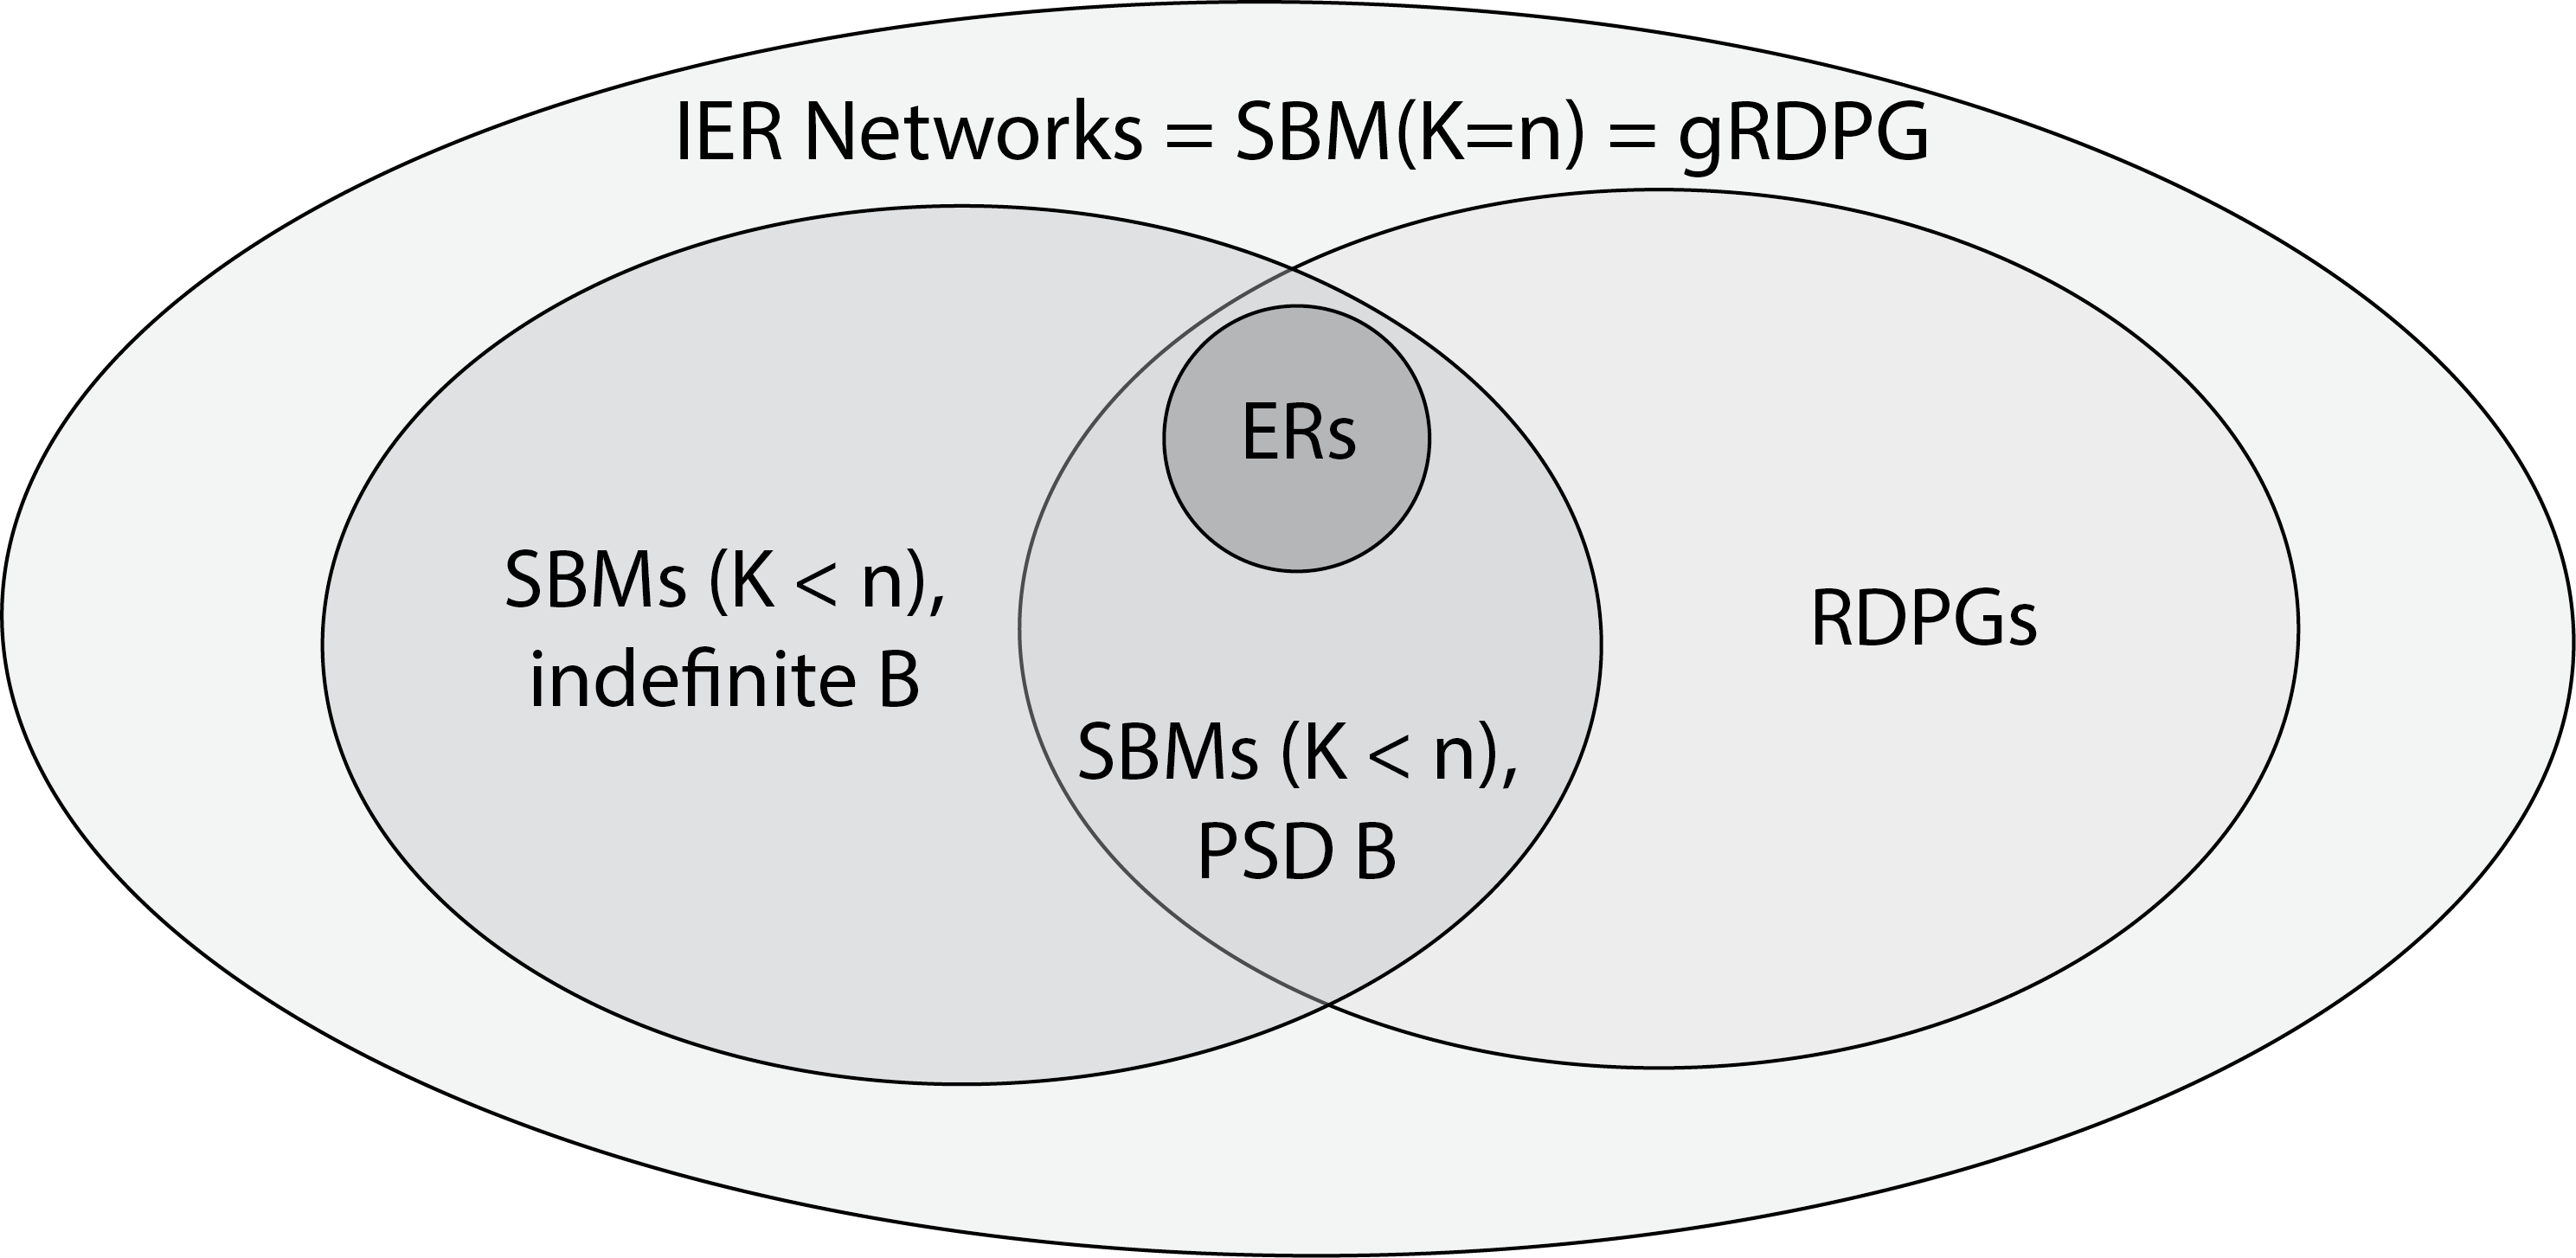
\includegraphics[width=\linewidth]{representations/ch5/Images/unify_sn.png}
    \caption{The hierarchy of complexity for Random Network Models.}
    \label{fig:ch5:hierarchy}
\end{figure}

\subsection{Read on for more}

If you want a deeper level of technical depth on Inhomogeneous Erd\"os R\'enyi Random Networks, please see Appendix \ref{app:ch12:rdpg}.


\newpage